%!TEX root = ../main.tex
\chapter{Experiments and Workflow}\label{chap:experiments}
本節では、主に実環境データを対象にした、屈折を考慮した水中3次元再構成のための完全なパイプラインとその実装を概説する。

% \begin{figure}[htbp]
%   \centering
%   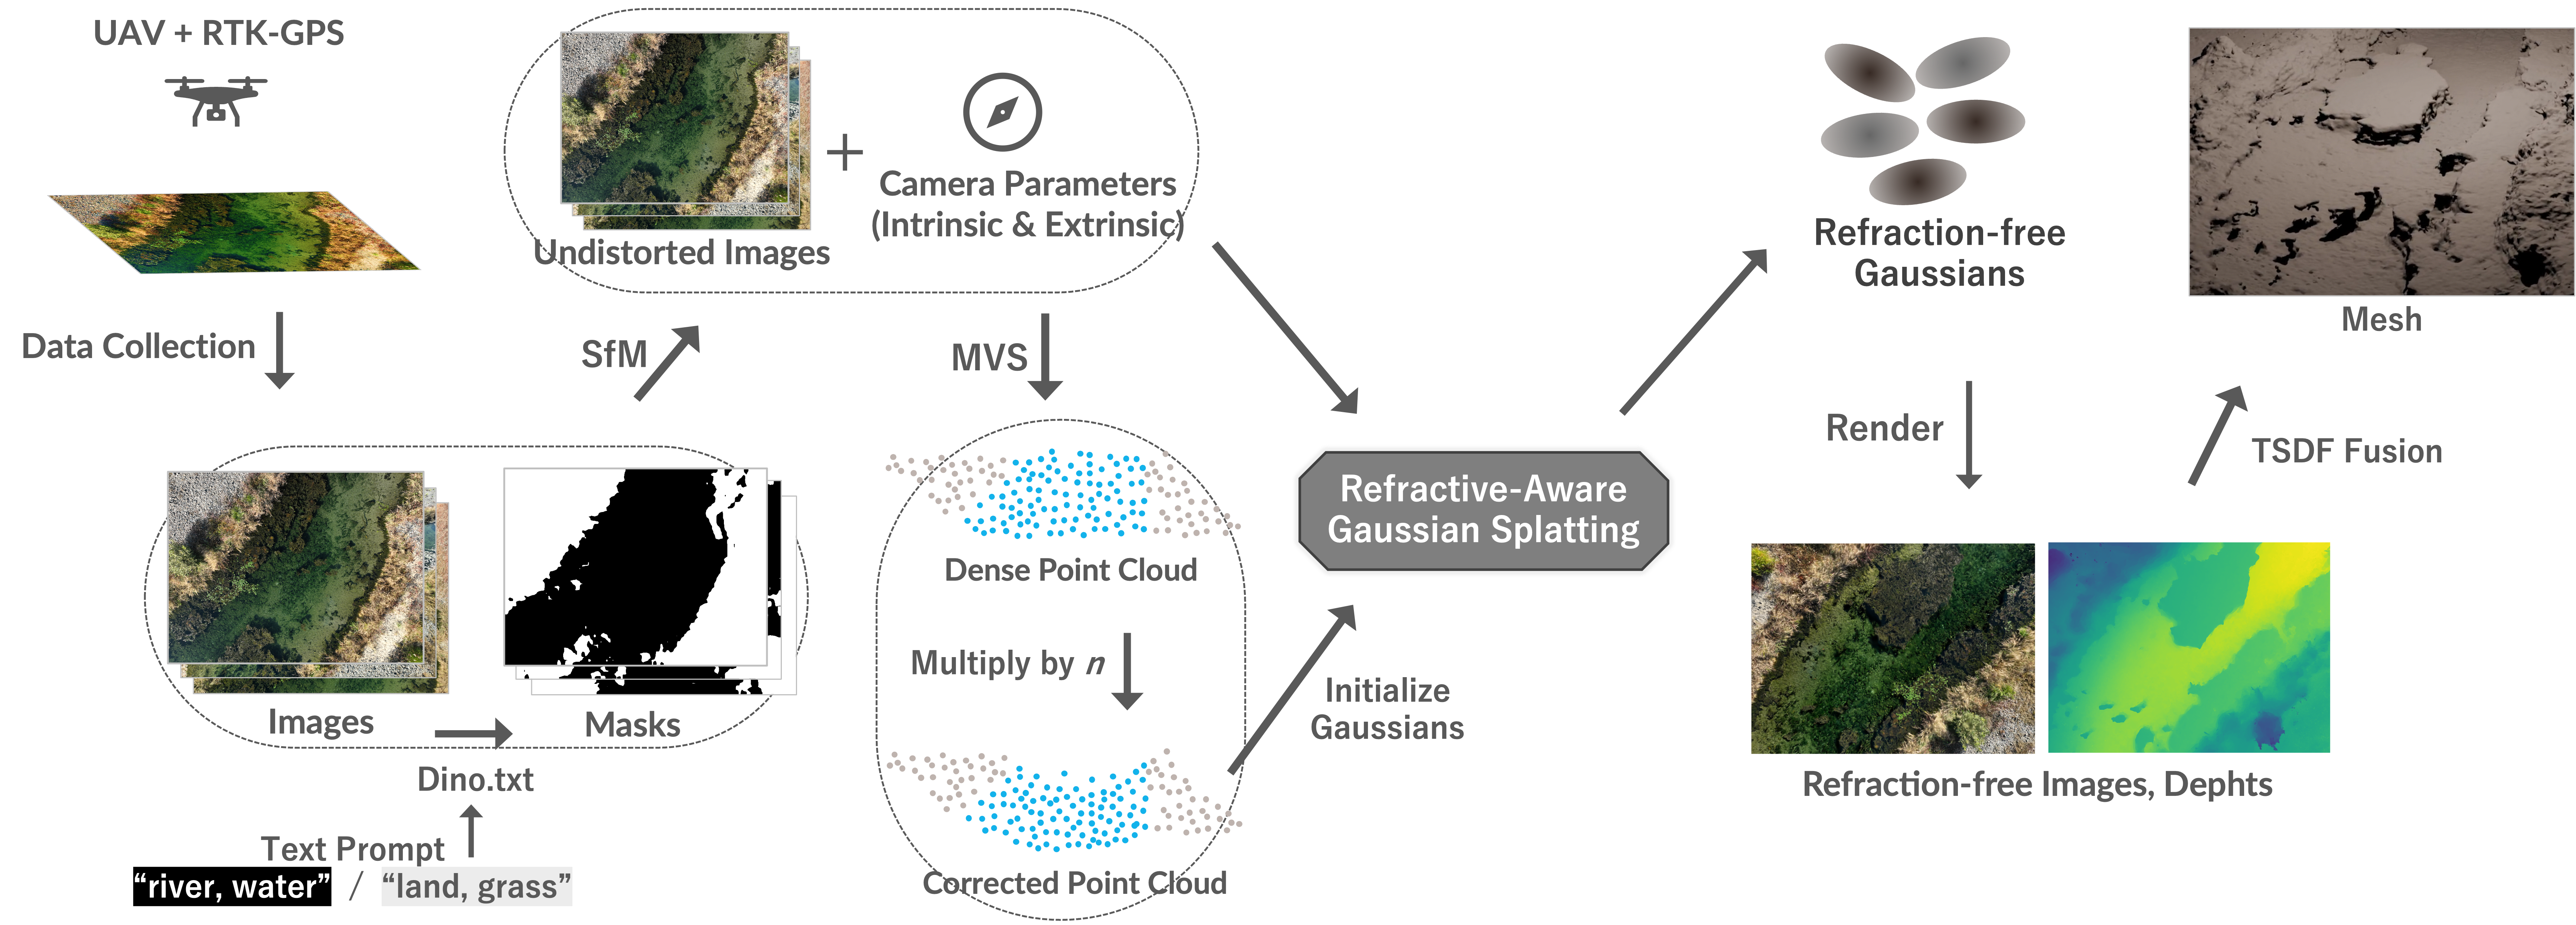
\includegraphics[width=0.95\textwidth]{figure/70_experim/workflow.png}
%   \caption{
%     実環境データを対象にした、屈折を考慮した水中3次元再構成のための完全なパイプライン。
%     }
%     \label{fig:workflow}
% \end{figure}

\begin{sidewaysfigure}[p]
  \centering
  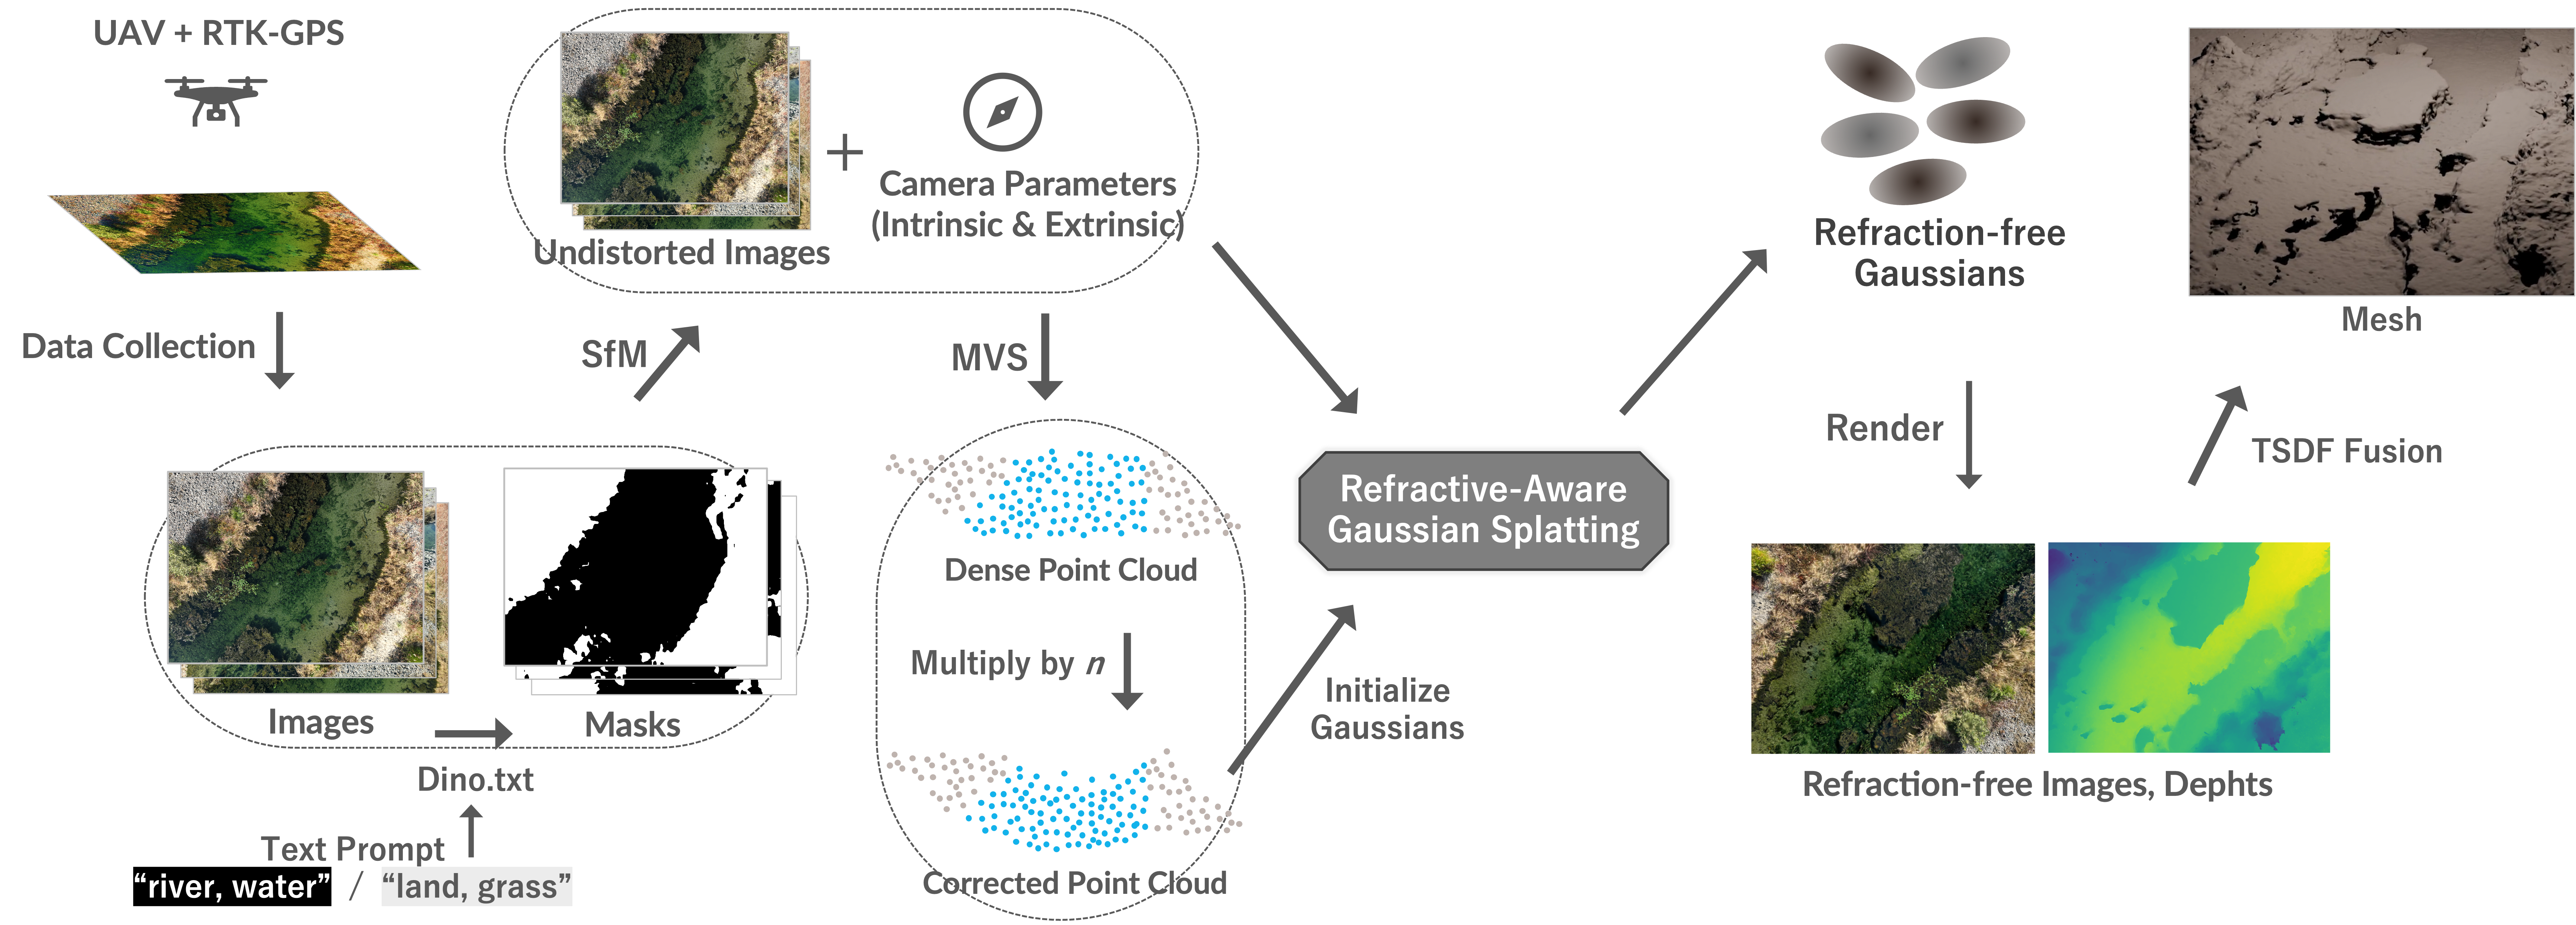
\includegraphics[width=0.95\textheight, keepaspectratio]{figure/70_experim/workflow.png}
  \caption{
    実環境データを対象にした、屈折を考慮した水中3次元再構成のための完全なパイプライン。
    }
  \label{fig:workflow}
\end{sidewaysfigure}

\note{Abstract図表をより詳細に説明する}

\section{Camera Calibration}\label{sec:camera-calibration}

RA-GSは、他の他視点三次元再構成タスク(\cref{subsec:mvs,subsec:nvs})と同様に、正確なカメラ内部・外部パラメータと歪みのない画像(Undistorted Images)を必要とする。
これらは、COLMAP~\cite{schoenberger2016_colmap}などのSfM(\cref{subsec:sfm})によって推定することが標準となっている。
本研究では、学術研究に無料で使用できるフォトグラメトリソフトウェアRealityScan\cite{RealityScan}を用い、カメラキャリブレーションと画像の歪み補正を行った。
\cref{sec:field-dataset}で示したように、スケール不定性を持つ多視点画像による再構成に対し、高精度なRTK-GPSの位置情報をリファレンスに用いることで、実環境に即したスケールを保証する。

陸域を十分に撮像できず、後続の水面マスク抽出手法が適用できない場合は、R-SfM\cite{Makris2024_refractive-aware-sfm}を用いて、屈折領域込みでのカメラポーズ推定が可能である。
また、RA-GSでは、カメラ外部パラメータに関しての勾配も追跡可能で、Photometricな情報からのカメラポーズ推定も可能であり、予め使用するカメラの内部キャリブレーションを行っておくことで、ジオリファレンス情報や屈折により誤差の増加したSfMによるカメラ位置姿勢を初期値として、シーンと同時にカメラ姿勢を最適化していくことも可能である。

\section{Mask Generation by Vision-Language Models}\label{sec:mask-generation}

本研究が対象とする空気中から水面下を対象としたシーンにおいては、光の屈折により、
やはりSfMが前提とする光の直進性が成立しなくなり、精度は悪化する
~\cite{she2024IROS_Refractive-COLMAP}。

\cite{she2024IROS_Refractive-COLMAP,Chadebecq2017ICCV_Refractive-Structure-from-Motion,Sedlazeck2013ICCV_Refractive-Structure-from-Motion,Makris2024_refractive-aware-sfm}
など、明示的に屈折を考慮したSfMは提案されているが、RA-GSの性能を最大限正確に検証するため、本研究では水面をマスクすることで、陸域のStaticなSceneのみを用いて特徴点検出から始まるSfMプロセスを行い、正確なカメラパラメータを推定する。
これは、一般のシーンの三次元復元でも一般的な手法であり、陸域であれば、人物や車両などの移動体、鏡などの反射物(Distractor)をマスクとして除外する機能は、RealityScanのみならず、COLMAPや他の商用フォトグラメトリソフトウェアでも同様の手法が実現可能である。
陸域で十分な特徴点を得られるように\cref{sec:field-dataset}で取得したUAV画像には十分な陸域が写っていることを確認した。


UAV画像から水面や Distractor を抽出するマスク生成には、以下のことがらが実務における効率の観点から求められる。

\begin{itemize}
  \item Automated:
    数十〜数百枚規模の UAV 画像に対して、オペレータが1枚ずつ手動ラベリングを行うことは現実的ではなく、
    自動的に大規模な画像データからマスクを生成できる必要がある。
  \item Robustness:
    水底の特性、季節・天候や時間帯によるシーンの変化、陸域・植生など、実フィールドにおける多様なシーンの構成要素に対して安定して頑健に対象のマスクを生成できる必要がある。
  \item Zero-Shot Adaptability:
    自動化を実現するための深層学習モデルに対し、現場ごとに追加のアノテーションや再学習を行うことは、手動ラベリングと同様の多大なコストを要する。
    多様な現場に対して、同一のモデルを適応させることができることが望ましい。
  \item Controllability:
    「water surface」「boat」「people」といった自然言語のプロンプトを用いて、環境内の対象クラスを柔軟に切り替えられることは、
    RobustnessやZero-Shot Adaptabilityの根底にある要件であり、高いインタラクティビティを提供する。
\end{itemize}

これらの要件を満たすべく本研究では、オープン語彙物体検出モデル(DINO.txt\cite{Jose2025CVPR_DINOv2-Text,Simeoni2025_DINOv3})を利用し、テキストプロンプトによるゼロショット・セグメンテーションを行う。
DINO.txtの概要は\cref{fig:DinoTXT}に示す。
\note{
  Dino.txtの簡単な説明。
  Dinoによる豊かな特徴量を、Text と "Ground"させることで、自然言語によるセマンティックセグメンテーションが可能な時代だっちゃ。
}



\begin{figure}[htbp]
  \centering
  \includegraphics[width=0.95\textwidth]{figure/70_experim/DinoTXT.png}
  \caption{
    Dino.txtの概要。
    \cite{Jose2025CVPR_DINOv2-Text}から引用。\\
    (左):DinoV2\cite{Oquab2023_DINOv2}による自己教師あり学習(Self-Supervised Learning: SSL)による特徴量の主成分分析による可視化。
     (本研究では、DinoV3\cite{Simeoni2025_DINOv3}を使用している)
    (中央):学習済SSLと、ゼロから学習したテキストエンコーダを整合させるトレーニング戦略。
    視覚エンコーダ上に軽量なビジョンブロックを追加することで、テキストとの整合性をさらに向上させている。
    モデル全体はわずか5万イテレーションで学習可能であり、ゼロショット分類およびオープン語彙セグメンテーションの両タスクにおいて高い性能を有する。
    (右):出力結果例。(入力画像と、対応する zero-shot分類や open-vocabularyセグメンテーションの結果)。
    }
    \label{fig:DinoTXT}
\end{figure}

\missingfigure{実際のマスク作成例。定量も含めて示す}

実環境データ~\cref{sec:field-dataset}に対しては、DinoV3\cite{Simeoni2025_DINOv3}のリポジトリで公開されている学習済みモデル\footnote{\url{https://ai.meta.com/resources/models-and-libraries/dinov3-downloads/}}およびコード\footnote{\url{https://github.com/facebookresearch/dinov3/blob/main/notebooks/dinotxt_segmentation_inference.ipynb}}を利用し、水域と陸域を区別するマスクを生成した。
水面はマスクにより除外し(0値)、陸域には陸地や草木などが含まれ、それらを非マスクとして残す(1値)。
今回は非マスクとして扱ったが、風の強い日では草木は揺らめくことで幾何推定の精度が悪化するため、その場合はマスクとして除外する必要があるといった多様な環境・状況に対してのControllabilityが必要となる。
宇治川データセットでは水面に多数の浮遊植物が凝集して存在し、それらは屈折の影響を受けず、SfMによる幾何推定の精度向上に寄与すると考えたため、明示的にプロンプトで指定することで除外を試みた。

まずは、UAVによる上空からの視点であることを補強するテンプレート(例: \texttt{a drone view of \{\}.})を作成した。
これは、一般に多くの基盤モデルは地上からの視点を想定してGroundingされているため、上空からの視点を補強することで、より精度の高いマスク生成が可能となると考えられる。



\begin{figure}[htbp]
  \centering 
  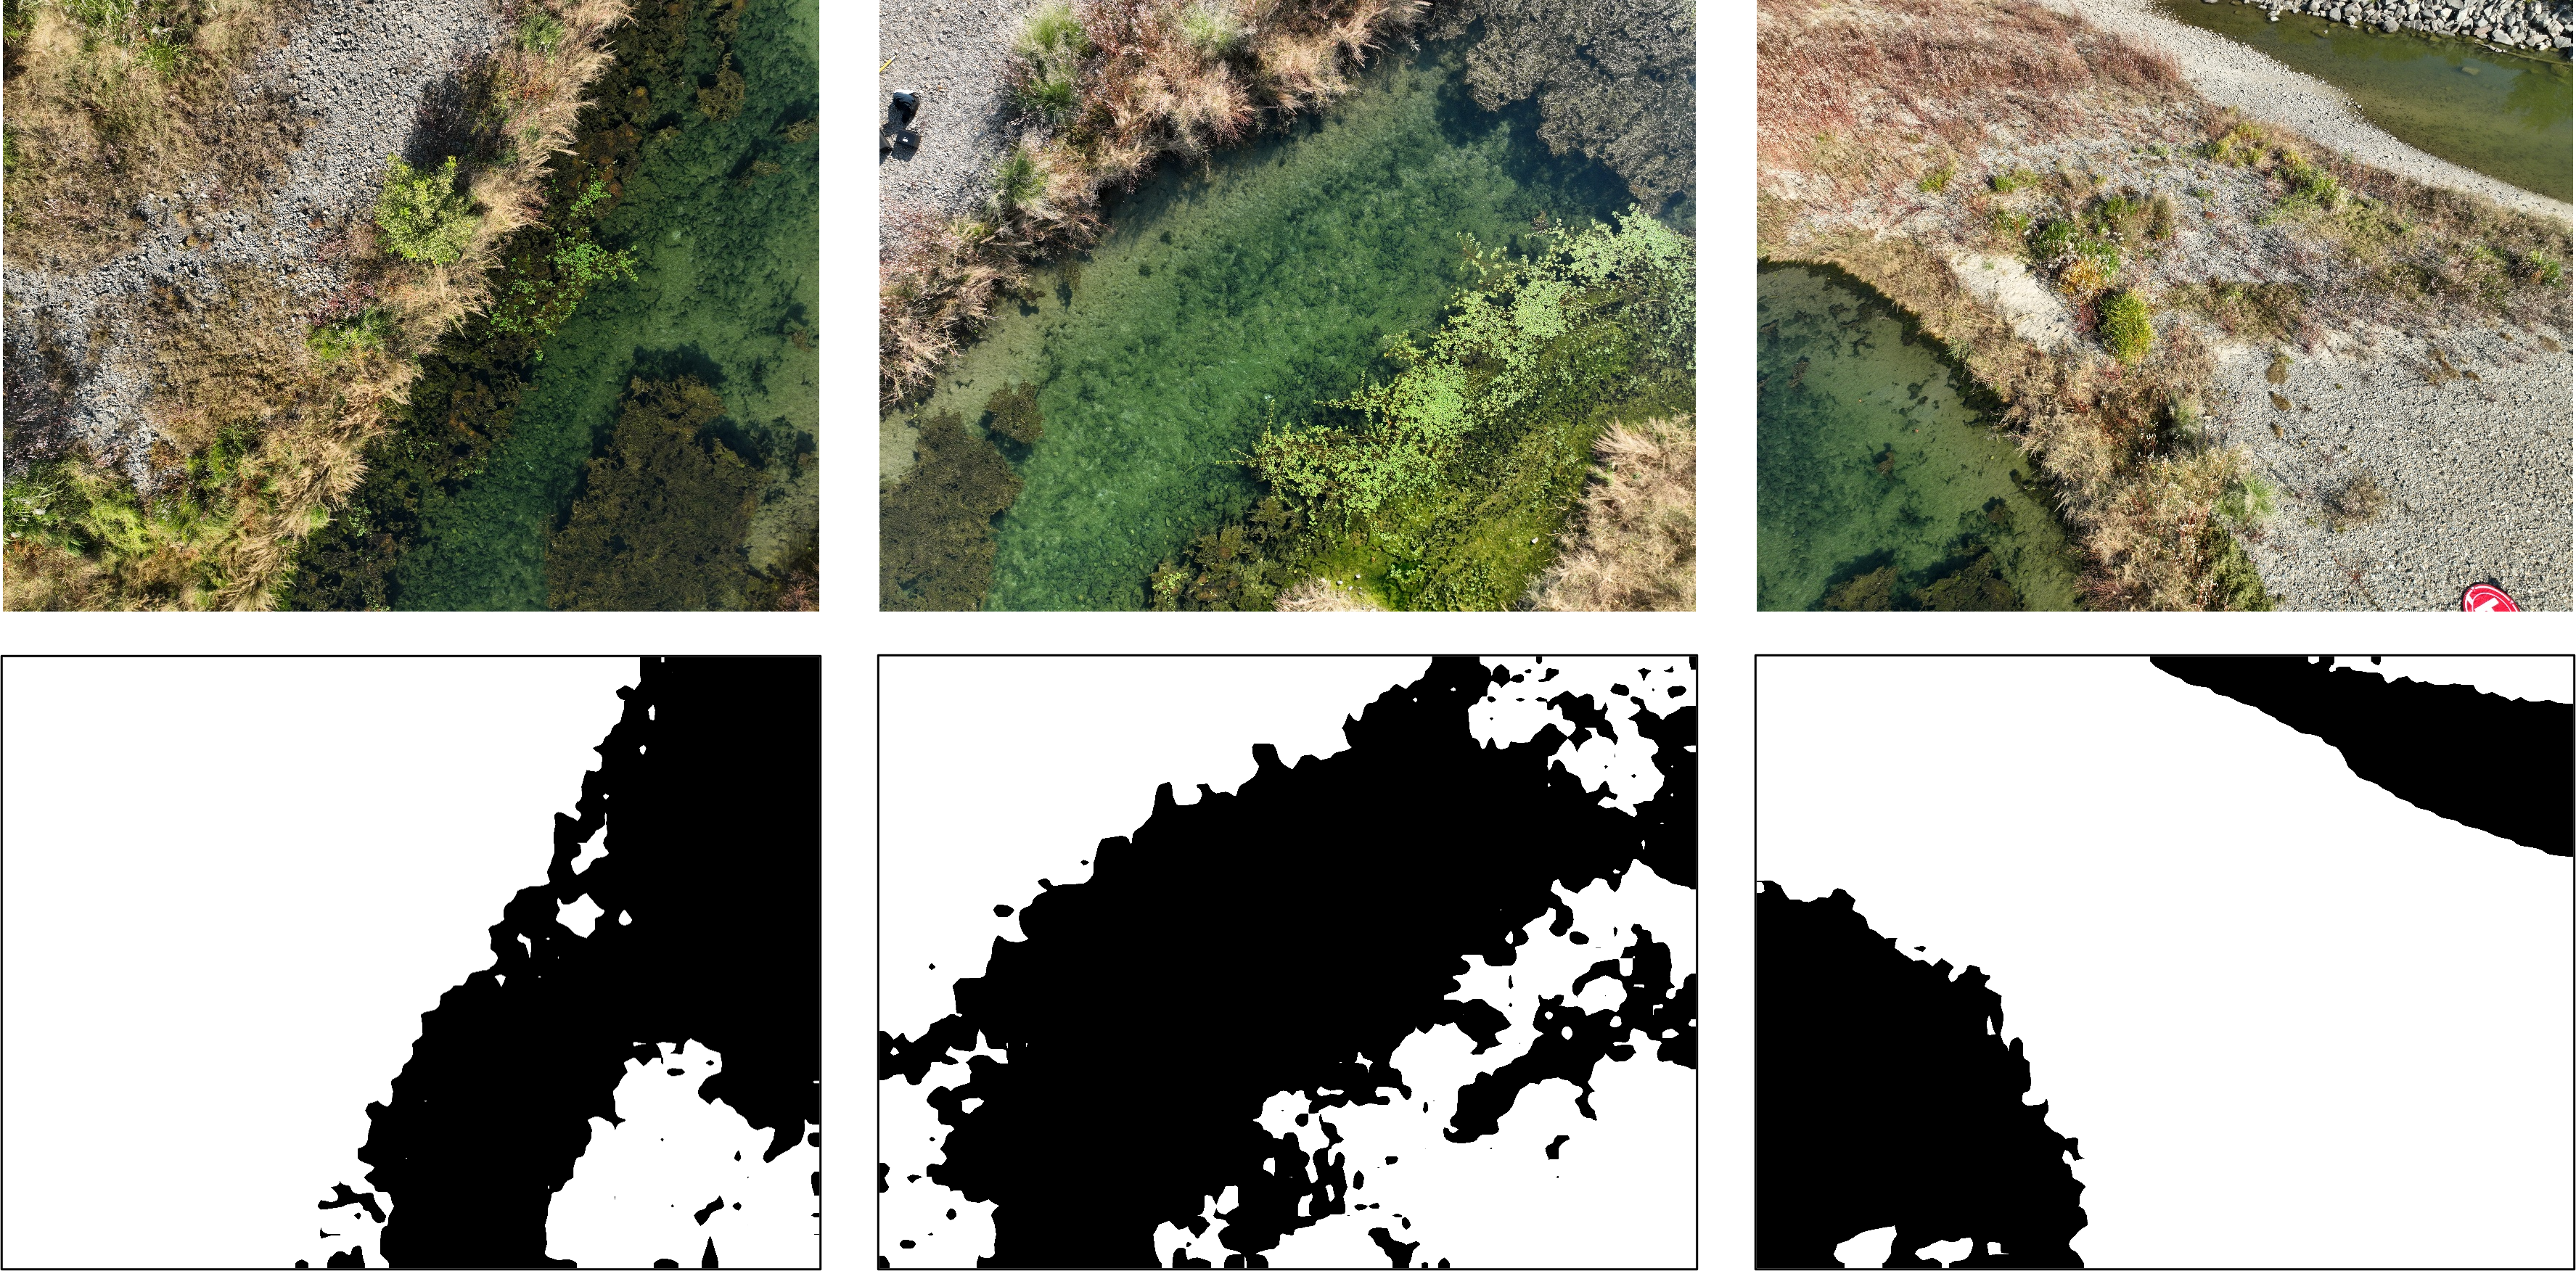
\includegraphics[width=0.90\textwidth]{figure/70_experim/mask-result.png}
  \caption{Area1におけるマスク生成結果}
  \label{fig:mask-result}
\end{figure}


\begin{algorithm}[htbp]
  \SetAlgoLined
  \DontPrintSemicolon
  \caption{DINO.txtによるセグメンテーションの推論手順}
  \label{alg:segmentation}
  
  \KwIn{\\
    \Indp
    Input images $\mathcal{I}$ \\
    Text prompts $\mathcal{P} = \{P_c\}_{c=1}^{C}$ mapped to $C$ categories (Water, Land, Veg)\\
    Pretrained Encoder Model $\Phi$\\
    \Indm
    }
  \KwOut{\\
   \Indp
    Segmentation masks $\mathcal{M}$\\ 
    \Indm
    }
  \BlankLine
  
  \tcp{Stage 1: Build Text Embeddings}
  Initialize text embeddings $\mathbf{T} \leftarrow \emptyset$, 
  Category map $\mathbf{C}_{map} \leftarrow \emptyset$\;
  \ForEach{category $c \in \{1, \dots, C\}$}{
      \ForEach{prompt $p \in P_c$}{
          Generate templates $\mathcal{T}_p = \{ \text{template}(p) \}$\;
          Extract features: $\mathbf{f}_p = \text{Normalize}(\text{Mean}(\Phi_{\text{text}}(\mathcal{T}_p)))$\;
          $\mathbf{T} \leftarrow \mathbf{T} \cup \{ \mathbf{f}_p \}$\;
          $\mathbf{C}_{map}[p] \leftarrow c$\;
      }
  }
  Stack $\mathbf{T} \in \mathbb{R}^{N \times D}$ where $N$ is total prompts\;
  \BlankLine

  \tcp{Stage 2: Image-Text Matching}
  \ForEach{image $I \in \mathcal{I}$}{
      Preprocess image: $I_{in} \leftarrow \text{Resize}(I)$\;
      Extract image features: $\mathbf{F} = \Phi_{\text{image}}(I_{in})$\;
      Compute logits: $\mathbf{L} = s \cdot \mathbf{F} \cdot \mathbf{T}^\top$ \tcp*{$s$ is a scaling factor}
      Upsample logits to original size: $\mathbf{L}_{up} \leftarrow \text{Bilinear}(\mathbf{L})$\;
      Compute probabilities: $\mathbf{P}_{all} \leftarrow \text{Softmax}(\mathbf{L}_{up})$\;
      \BlankLine
      
      \tcp{Stage 3: Aggregation by Category}
      Initialize final probabilities $\mathbf{P}_{final} \in \mathbb{R}^{C \times H \times W}$\;
      \For{$c = 1$ \KwTo $C$}{
          Identify indices: $\mathcal{K}_c = \{k \mid \mathbf{C}_{map}[k] = c\}$\;
          Extract detailed probs: $\mathbf{P}_{sub} = \mathbf{P}_{all}[\mathcal{K}_c]$\;
          Aggregate: $\mathbf{P}_{final}[c] \leftarrow \text{AGG}(\mathbf{P}_{sub})$ \tcp*{Sum of probabilities }
      }
      \BlankLine

      \tcp{Stage 4: Prediction \& Save}
      Generate mask: $M \leftarrow \arg\max_{c} (\mathbf{P}_{final})$\;
      Save $M$
  }
\end{algorithm}

具体的なマスクのアルゴリズムは\cref{alg:segmentation}の通りである。
本手法では、ターゲットとなる $C$ 個のクラス(Water, Land, Vegetation)に対し、それぞれ複数のテキストプロンプト $\mathcal{P}_c$ を用意し(\cref{tab:prompts})、これらに前述のテンプレートを適用してテキストエンコーダに入力することで、テキスト埋め込みベクトル $\mathbf{T}$ を事前に構築する。
推論時には、入力画像 $I$ を画像エンコーダに通して空間特徴量 $\mathbf{F}$ を抽出し、テキスト埋め込み$\mathbf{T}$との内積をとることで、各画素とプロンプトとの類似度を算出する。
DinoV3の特徴マップは入力画像よりも解像度が低いため、バイリニア補間により元の画像サイズへアップサンプリングを行った後、Softmax関数により確率スコア$\mathbf{P}$に変換する。
そして、同一カテゴリに属する複数のプロンプトに対する確率スコアを合算(Aggregation)する
\footnote{Softmax関数を事前に適用しているため、合算に加算を用いることは数学的に妥当であり、カテゴリ内の要素数にフェアな確率を生成する。}。
最終的に、画素ごとに確率が最大となるカテゴリを選択することで、ピクセル単位のセマンティックマスク $\mathcal{M}$ を生成した。
これにより、水面領域(Water)と、再構成に使用する陸域(Land/Vegetation)を自動かつロバストに分離することが可能となる。


\begin{table}[htbp]
  \centering
  \caption{
    Area1における水面マスク抽出に用いたテキストプロンプト。\\
    浮遊植物と水域・陸域を区別しやすいように3カテゴリで分類を行った。
    テンプレートは、UAVによる上空からの視点を強調するものである。
  }
  \label{tab:prompts}
  \begin{tabular}{lp{0.7\linewidth}}
    \hline
    カテゴリ & プロンプト(英語キーワード) \\
    \hline
    水(除外対象/マスク) &
      \texttt{river}, \texttt{lake}, \texttt{sea},
      \texttt{river water},
      \texttt{blue water},
      \texttt{green water},
      \texttt{water surface},
      \texttt{ripples},
      \texttt{reflection},
      \texttt{stream},
      \texttt{fluid},
      \texttt{riverbeds} \\
    \hline
    陸地(抽出対象1) &
      \texttt{sand},
      \texttt{gravel},
      \texttt{pebbles},
      \texttt{dirt},
      \texttt{mud},
      \texttt{dry land},
      \texttt{rock}, \texttt{stone},
      \texttt{boulder},
      \texttt{concrete},
      \texttt{shore},
      \texttt{ground},
      \texttt{reef},
      \texttt{sandbank},
      \texttt{sandy spit},
      \texttt{shoal} \\
    \hline
    植生(抽出対象2) &
      \texttt{vegetation},
      \texttt{grass},
      \texttt{tree}, \texttt{bush},
      \texttt{leaves},
      \texttt{plant},
      \texttt{leaves on the water surface},
      \texttt{green scum},
      \texttt{floating weeds},
      \texttt{water plants},
      \texttt{lily pads} \\
    \hline
    テンプレート & 
      \texttt{a drone view of \{\}.}
      \texttt{an aerial view of \{\}.}
      \texttt{a top-down photo of \{\}.}
      \texttt{a photo of the \{\}.}
      \texttt{\{\} texture.}
      \texttt{a close-up of \{\}.}
      \texttt{a view of \{\} from above.}
      \texttt{an overhead view of \{\}.}
      \texttt{a bird's-eye view of \{\}.}
      \texttt{a high-angle shot of \{\}.} 
      \texttt{an orthophoto of \{\}.} \\
    \hline
  \end{tabular}
\end{table}


\newpage

\section{Initialization of Gaussians}\label{sec:initialization-of-gaussians}

\begin{figure}[htbp]
  \centering
  \includegraphics[width=0.75\textwidth]{figure/70_experim/sfm-random_3dgs.png}
  \caption{
    Gaussianの初期化による比較。
    \cite{Kerbl2023ToG_3DGS}から引用。\\
    上:ランダムな点群による初期化\\
    下:SfM点群による初期化\\
    SfM点群による初期化は再構成精度向上に有効であることを示している。
    特にカバーされる視点の少ない背景領域で顕著である。
    }
    \label{fig:initialization-of-gaussians}
\end{figure}


Gaussian Splattingでは、SfMから得られた粗点群の位置をもとにGaussianを初期化するが、もしこれをこれをランダムな位置で初期化した場合、再構成の品質が低下することが示されている(\cref{fig:initialization-of-gaussians})。
本環境でも同様で、水面をマスクしたSfMプロセスからは、水底の点群を得ることができず、河床の再構成の質が大幅に低下する(\cref{fig:init-ablation-bed})。

\IncludeTwoImages[6cm]
  {figure/70_experim/GS-riverbed-w-ini.png}{川底の点群を入力した場合の再構成結果}
  {figure/70_experim/GS-riverbed-wo-ini.png}{川底の点群を入力しなかった場合の再構成結果}
  {
    川底の点群を入力した場合と入力しなかった場合の再構成結果の比較。\\
    学習は3DGSによる結果である。
    川底に補正点群を設けない場合、川底のシーンの質は大幅に低下する。
  }
  {fig:init-ablation-bed}

そこで、本研究では、水面をマスクしたSfM処理の後に、マスク化を解除し、推定したカメラパラメータからMVS(\cref{subsec:mvs})を行い、川底の点群を生成した。
屈折の影響により優れた質の点群を生成できず、初期化のための点群であるから、時間効率を踏まえた低い品質のパラメータで行うことが可能である。
この生成点群に対し、\cite{Woodget2014_PhotograBathy-multiply-n,westaway2001_PhotograBathy-multiply-n}で報告される水面下の点群に対し屈折率$n=1.33$を乗することで、補正点群を生成した。
後述するRA-GSで保持できるGaussian数(点群数)にメモリ容量上の制約があるため、RA-GSの初期化においてはこの点群をさらにダウンサンプリングして用いた。
具体的には、12GBのVRAMを搭載したNVIDIA RTX 3090 GPUでは、最大で約3M個のGaussianを保持できるため、初期化には約500k個のGaussianを用いるようにダウンサンプリングした。
\note{もう一度、実装して実験し直したほうがいい。2DGSの結果は、色を失った黒点群を使っていた。}






